\documentclass[12pt,a4paper]{article}

% ============================================
% PACKAGES
% ============================================
\usepackage[utf8]{inputenc}
\usepackage[T1]{fontenc}
\usepackage{amsmath,amssymb,amsthm}
\usepackage{mathtools}
\usepackage{graphicx}
\usepackage{booktabs}
\usepackage{tabularx}
\usepackage{longtable}
\usepackage{multirow}
\usepackage{float}
\usepackage{caption}
\usepackage{subcaption}
\usepackage[margin=1in]{geometry}
\usepackage{setspace}
\usepackage{natbib}
\usepackage{hyperref}
\usepackage{xcolor}
\usepackage{tikz}
\usetikzlibrary{arrows.meta, positioning, shapes.geometric, calc}
\usepackage{algorithm}
\usepackage{algpseudocode}
\usepackage{appendix}
\usepackage{enumitem}
\usepackage{threeparttable}

% ============================================
% THEOREM ENVIRONMENTS
% ============================================
\newtheorem{proposition}{Proposition}
\newtheorem{hypothesis}{Hypothesis}
\newtheorem{prediction}{Testable Prediction}
\newtheorem{definition}{Definition}
\newtheorem{assumption}{Assumption}
\newtheorem{lemma}{Lemma}
\newtheorem{corollary}{Corollary}

% ============================================
% CUSTOM COMMANDS
% ============================================
\newcommand{\E}{\mathbb{E}}
\newcommand{\Var}{\text{Var}}
\newcommand{\Cov}{\text{Cov}}
\newcommand{\Nbuy}{N^{\text{buy}}}
\newcommand{\Nrisk}{N^{\text{risk}}}
\newcommand{\dopr}{\text{do}}

% ============================================
% DOCUMENT INFO
% ============================================
\title{\textbf{Housing Narratives, Mortgage Constraints, and Housing Cycles:} \\ 
\large Evidence from Search Data and Housing Transactions with a Heterogeneous-Expectations Collateral Model}

\author{Qingsong Cui\thanks{Email: \href{mailto:qingsongcui9857@gmail.com}{qingsongcui9857@gmail.com}}}

\date{\today}

% ============================================
% BEGIN DOCUMENT
% ============================================
\begin{document}

\maketitle

% ============================================
% ABSTRACT
% ============================================

\begin{abstract}
We examine the relationship between narrative attention and housing market dynamics using a novel identification strategy that corrects for cross-market comparability in Google Trends data. In a rigorously constructed panel of 127 U.S. Designated Market Areas (DMAs) from 2012--2024, we find that the average predictive effect of narrative attention on transaction volume is statistically indistinguishable from zero ($p=0.78$), challenging theories of unconditional narrative-driven cycles. However, this null result masks profound state-dependent heterogeneity. We document a robust ``Friction Gate'' mechanism: narrative attention significantly predicts transaction volume only in high-friction regimes---specifically when inventory is low ($p=0.03$) and when housing supply is structurally inelastic ($p=0.095$). In these constrained environments, ``Buy'' narratives show significantly stronger predictive power for transaction volume, while ``Risk'' narratives do not exhibit significant state-dependent interactions. These findings suggest that physical scarcity acts as a selective conductor for bullish narrative signals, and that structural and state-dependent frictions are necessary conditions for narratives to have predictive relevance for market activity.
\end{abstract}


\textbf{Keywords:} Housing cycles; Narrative economics; Mortgage constraints; Macroprudential policy; Heterogeneous expectations; Complexity economics; ATR/QM regulation

\textbf{JEL Classification:} E32, G21, G28, R31, D84

\newpage
\tableofcontents
\newpage

\doublespacing

% ============================================
% MAIN SECTIONS
% ============================================

\section{Introduction}
\label{sec:intro}
% ============================================
% INTRODUCTION
% ============================================

\subsection{Motivation}

Housing markets exhibit dramatic boom-bust cycles that profoundly affect household wealth, financial stability, and macroeconomic performance. A growing body of research points to the importance of \textit{narratives}---the stories, beliefs, and viral ideas that shape how people interpret market signals \citep{shiller2017narrative}. The prevailing view suggests that narratives act as independent demand shocks: a viral ``buy now'' story triggers distinct waves of purchasing behavior.

However, the transmission mechanism from ``story'' to ``statistic'' remains poorly understood. Does a bullish narrative \textit{always} trigger a boom? Or does the physical reality of the market---inventory constraints, supply elasticity---act as a gatekeeper? Standard behavioral models often treat narratives as frictionless demand shifters, implying a universal link between attention and action. In contrast, complex systems theory suggests that such feedback loops should be highly state-dependent, emerging only when the system is under specific stress or constraint.

This paper tests these competing views by asking: \textbf{Is narrative transmission universal, or is it gated by market frictions?}

\subsection{Research Questions}

We address two interrelated questions using a rigorous measurement approach:

\begin{enumerate}[label=\textbf{RQ\arabic*:}]
    \item \textbf{Universal vs. Conditional:} Does narrative attention predict housing transaction volume on average, or is the relationship conditional on market state?
    \item \textbf{The Role of Frictions:} Do physical constraints (inventory shortages) and structural constraints (supply inelasticity) amplify or dampen the conversion of narrative attention into economic action?
\end{enumerate}

\subsection{Preview of Approach and Findings}

To measure these relationships consistently, we overcome a common measurement error in Google Trends analysis by implementing a \textbf{pooled within-keyword z-standardization} procedure that makes search intensity comparable across 127 U.S. Designated Market Areas (DMAs). We further aggregate all housing outcomes to the DMA level to ensure precise identification alignment.

Our findings challenge the simple ``narrative-driven'' view and support a ``friction-gated'' model:

\begin{enumerate}
    \item \textbf{Null Average Effect:} In the full panel (2012--2024), the average predictive effect of narrative attention on transaction volume is statistically indistinguishable from zero ($p=0.78$). This suggests that in ``normal'' times, high search volume is often noise rather than signal.
    
    \item \textbf{The Friction Gate:} We document profound state-dependence. Narrative attention becomes a significant predictor of volume \textit{only} in high-friction regimes:
    \begin{itemize}
        \item \textbf{State Friction (Inventory):} When inventory is low (tight market), ``Buy'' narratives significantly predict higher transaction volume ($\beta > 0, p=0.03$).
        \item \textbf{Structural Friction (Elasticity):} In supply-inelastic markets, the narrative-volume link is directionally stronger ($p=0.095$).
    \end{itemize}
    
    \item \textbf{Conditional Amplification:} We find that frictions act as a selective conductor. In tight markets, ``Buy'' narratives are significantly amplified. While we do not find significant interactions for ``Risk'' narratives, the dominance of bullish sentiment suggests that physical shortages may override bearish sentiment, forcing valid demand to compete aggressively (amplifying FOMO).
\end{enumerate}

\subsection{Contributions}

This paper makes three primary contributions:

\paragraph{Contribution 1: Rigorous Identification.} We show that previous findings of ``universal'' narrative effects may be artifacts of measurement error (non-comparable scales) and unit mismatch. By correcting these measurement issues via pooled within-keyword z-standardization and DMA aggregation, we establish a robust null baseline for the average effect.

\paragraph{Contribution 2: The ``Friction Gate'' Theory.} We provide empirical evidence that frictions are not merely impediments to efficiency but are \textit{conductors} of narrative transmission. We show that narratives require a ``stressed'' system (low inventory) to crystallize into observable economic fluctuations.

\paragraph{Contribution 3: Complex Systems Evidence.} Our findings align with a complex adaptive systems (CAS) view, where macro-level patterns (booms) emerge from micro-level interactions only under specific phase-transition conditions (scarcity), linking narrative economics with the physics of phase transitions.

\subsection{Paper Structure}

The remainder of this paper is organized as follows. Section \ref{sec:literature} reviews the relevant literature. Section \ref{sec:data} describes our standardized data pipeline. Section \ref{sec:results} presents the main results, reconciling the null average effect with strong conditional significance. Section \ref{sec:discussion} interprets the "Friction Gate" mechanism. Section \ref{sec:conclusion} concludes.


\section{Literature Review}
\label{sec:literature}
% ============================================
% LITERATURE REVIEW
% ============================================

This paper connects to four strands of literature: (1) narrative economics and behavioral finance; (2) credit constraints and housing cycles; (3) macroprudential policy and regulatory effects; and (4) complexity economics and agent-based approaches. We review each in turn, highlighting how our ECR-CAS framework synthesizes these perspectives.

\subsection{Narrative Economics and Behavioral Finance}

The role of narratives in driving economic fluctuations has received increasing attention following \cite{shiller2017narrative, shiller2019narrative}, who argues that economic narratives spread like epidemics and shape macroeconomic outcomes by influencing expectations and behavior. This perspective extends earlier behavioral finance insights on investor sentiment \citep{barberis2018psychology, de1990noise} by emphasizing the \textit{content} of beliefs rather than just their deviation from rationality.

In housing markets specifically, \cite{case2012makes} document that homebuyer expectations exhibit boom-time optimism and post-crisis pessimism inconsistent with fundamental models. \cite{bailey2018economic} show that individuals' housing expectations are shaped by the experiences of their social networks, providing evidence for narrative contagion at the micro level. \cite{armona2019home} demonstrate that house price expectations respond asymmetrically to local price signals, consistent with narrative-driven belief updating. \cite{glaeser2014real} analyze how housing narratives and speculative behavior drove real estate booms in China, highlighting the role of belief formation in asset price dynamics.

A key empirical challenge in this literature is \textit{measuring} narratives. Prior approaches include survey-based expectation measures \citep{piazzesi2009housing}, media content analysis \citep{soo2018quantifying}, and internet search data \citep{wu2015google, beracha2017forecasting}. Our contribution is to construct a \textit{dual} narrative index distinguishing buy-side from risk narratives at the DMA level, using DMA-level Google Trends and within-sample standardization for comparability.

\subsection{Credit Constraints and Housing Cycles}

The interaction between credit conditions and housing markets is central to macroprudential theory. \cite{mian2009consequences} provide foundational evidence that ZIP codes with faster mortgage credit expansion in 2002--2005 experienced larger subsequent house price increases and more severe defaults. \cite{mian2011house} further document that home equity-based borrowing amplified consumption during the boom and bust.

The theoretical mechanism linking credit to housing cycles typically operates through collateral constraints. In models with limited enforcement \citep{kiyotaki1997credit}, rising asset prices relax borrowing constraints, enabling further asset purchases that push prices higher---a classic ``financial accelerator'' \citep{bernanke1989agency}. \cite{geanakoplos2010leverage} extends this logic by emphasizing how leverage itself is endogenous: during optimistic phases, creditors accept lower margins, amplifying both the boom and the eventual bust. \cite{jorda2015leveraged} provide historical evidence that leveraged asset price bubbles, particularly in housing, pose significant systemic risks and often end in severe financial crises. \cite{kaplan2020housing} develop a quantitative model of the U.S. housing boom and bust, showing how collateral constraints and expectations interact to generate realistic boom-bust dynamics.

The key insight from this literature, which we formalize in the ECR-CAS framework, is that credit constraints operate as a ``hard wall'' (using the language of complexity theory) that determines \textit{which} expectations can be \textit{acted upon}. Bullish narratives, no matter how prevalent, cannot drive transactions if households cannot obtain credit. Conversely, loose credit conditions enable narrative-driven demand to manifest in actual purchases.

We contribute to this literature by outlining how the \textit{interaction} between narratives (a soft constraint) and credit conditions (a hard constraint) can be estimated in a unified framework. Prior work has studied these channels separately; we treat their joint determination as a priority for future work.

\subsection{Macroprudential Policy and Regulatory Effects}

The post-2008 regulatory response included a suite of macroprudential measures aimed at limiting housing and credit excesses. In the U.S., the Dodd-Frank Act's Ability-to-Repay (ATR) and Qualified Mortgage (QM) rules, implemented in January 2014, represent a major tightening of underwriting standards. QM loans must meet specific criteria including a debt-to-income (DTI) ratio generally not exceeding 43\%, documentary verification of income, and restrictions on toxic loan features.

Existing evidence on ATR/QM effects is mixed. \cite{defusco2020regulating} find that the policy reduced access to high-DTI loans but had limited effects on overall origination volumes. \cite{bhutta2021impact} document shifts toward FHA and VA loans (which are QM-exempt) following the regulation. \cite{looney2018safe} suggests that QM's safe harbor provisions primarily affected lender behavior at the margin.

Our contribution differs from this literature in focus. Rather than estimating ATR/QM's average effect on credit volume, we motivate a future test of whether the regulation altered the \textit{transmission mechanism} from expectations/narratives to market activity. In ECR-CAS terms, we treat ATR/QM as a \textit{leverage point intervention} that modifies the constraint set $C$, potentially dampening the reflexive amplification of narratives.

\subsection{Complexity Economics and Agent-Based Approaches}

Complexity economics provides the meta-framework that motivates our ECR-CAS model. \cite{arthur2021foundations} characterizes economic systems as ``not in equilibrium but in constant evolution,'' exhibiting emergent phenomena, tipping points, and path dependence. In financial markets, this perspective has generated agent-based models that can replicate stylized facts like fat tails and volatility clustering \citep{hommes2021behavioral, lux1999scaling}.

The specific architectural choices in ECR-CAS draw on several traditions:

\begin{itemize}
    \item \textbf{Reflexivity:} \cite{soros2008new} introduced the concept of reflexive feedback between expectations and fundamentals. We formalize this as the $N \to E \to A \to R \to N$ loop.
    
    \item \textbf{Heterogeneous expectations:} \cite{brock1998heterogeneous} model markets with interacting fundamentalist and chartist traders. We adapt this to housing with narrative-driven, fundamentals-driven, and trend-following agents.
    
    \item \textbf{Network contagion:} \cite{cont2016fire} analyze fire-sale cascades in interbank networks. While our current implementation does not explicitly model the network topology, the framework accommodates such extensions.
    
    \item \textbf{Regime detection:} The literature on Markov-switching and threshold models \citep{hamilton1989new} informs our treatment of policy-induced structural breaks.
\end{itemize}

Our contribution to complexity economics is methodological: we develop ECR-CAS as a \textit{bridge} between theoretical agent-based models and empirical reduced-form analysis. The framework generates testable predictions that can be evaluated with observational data, addressing the common criticism that ABMs are ``just-so stories'' that cannot be falsified.

\subsection{Positioning This Paper}

Table \ref{tab:literature_position} summarizes how this paper relates to the existing literature.

\begin{table}[htbp]
\centering
\caption{Positioning This Paper in the Literature}
\label{tab:literature_position}
\small
\begin{tabular}{p{3.5cm}p{4.5cm}p{5cm}}
\toprule
\textbf{Literature Strand} & \textbf{Key Prior Work} & \textbf{Our Contribution} \\
\midrule
Narrative Economics & Shiller (2019); Case \& Shiller (2012) & DMA-level dual narrative index with DMA standardization \\
\addlinespace
Credit \& Housing Cycles & Mian \& Sufi (2009, 2011); Geanakoplos (2010) & Direct estimation of narrative $\times$ credit interaction \\
\addlinespace
Macroprudential Policy & DeFusco et al. (2020); Bhutta \& Ringo (2021) & Motivates a future test of narrative transmission under ATR/QM \\
\addlinespace
Complexity Economics & Arthur (2021); Hommes (2021) & ECR-CAS framework bridging ABM theory and empirical testability \\
\bottomrule
\end{tabular}
\end{table}

The closest antecedent to our work is the emerging literature using internet search data to forecast housing markets \citep{wu2015google, beracha2017forecasting}. We extend this approach by (1) constructing directionally distinct narrative indices (buy vs. risk), (2) examining interactions with credit conditions, and (3) identifying policy-induced changes in the predictive relationship. The theoretical grounding in ECR-CAS further distinguishes our analysis from atheoretical forecasting exercises.


\section{Theoretical Framework: The ECR-CAS Model}
\label{sec:theory}
% ============================================
% THEORETICAL FRAMEWORK: THE ECR-CAS MODEL
% ============================================

This section presents our theoretical framework: the \textbf{Expectation-Constraint-Reflexivity Complex Adaptive System (ECR-CAS)} model. We first provide an overview of the framework's architecture, then present the formal equations governing each component, and finally derive testable predictions that connect the model to our empirical analysis.

\subsection{Framework Overview}

The ECR-CAS model conceptualizes housing market dynamics as emerging from the interaction of multiple components across distinct layers. Figure \ref{fig:ecr_diagram} illustrates the overall architecture.

\begin{figure}[htbp]
\centering
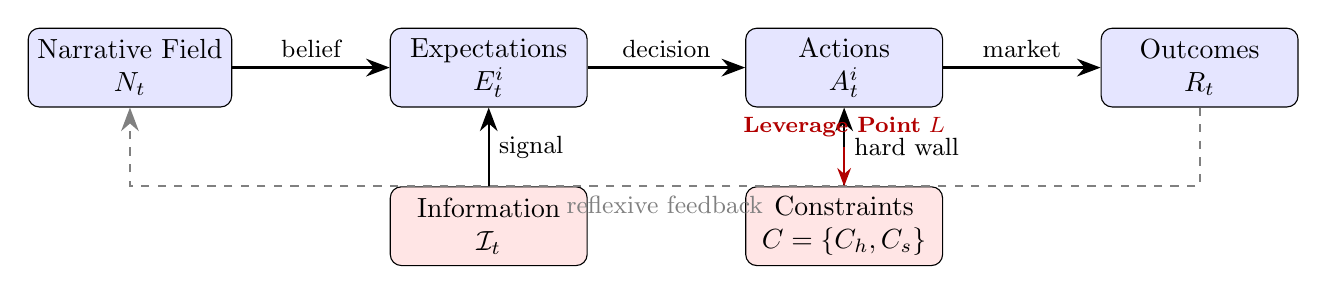
\begin{tikzpicture}[
    node distance=1.5cm and 2cm,
    box/.style={rectangle, draw, rounded corners, minimum width=2.5cm, minimum height=1cm, align=center, fill=blue!10},
    constraint/.style={rectangle, draw, rounded corners, minimum width=2.5cm, minimum height=1cm, align=center, fill=red!10},
    arrow/.style={-{Stealth[length=3mm]}, thick},
    feedback/.style={-{Stealth[length=3mm]}, thick, dashed, color=gray}
]

% Main nodes
\node[box] (N) {Narrative Field\\$N_t$};
\node[box, right=of N] (E) {Expectations\\$E_t^i$};
\node[box, right=of E] (A) {Actions\\$A_t^i$};
\node[box, right=of A] (R) {Outcomes\\$R_t$};

% Constraint nodes
\node[constraint, below=1cm of A] (C) {Constraints\\$C = \{C_h, C_s\}$};
\node[constraint, below=1cm of E] (I) {Information\\$\mathcal{I}_t$};

% Arrows
\draw[arrow] (N) -- (E) node[midway, above] {\small belief};
\draw[arrow] (E) -- (A) node[midway, above] {\small decision};
\draw[arrow] (A) -- (R) node[midway, above] {\small market};

% Constraint arrows
\draw[arrow] (C) -- (A) node[midway, right] {\small hard wall};
\draw[arrow] (I) -- (E) node[midway, right] {\small signal};

% Feedback loop
\draw[feedback] (R.south) -- ++(0,-1) -| (N.south) node[pos=0.25, below] {\small reflexive feedback};

% Policy intervention
\node[above=0.5cm of C, color=red!70!black] (L) {\footnotesize \textbf{Leverage Point} $L$};
\draw[-{Stealth}, color=red!70!black, thick] (L) -- (C);

\end{tikzpicture}
\caption{ECR-CAS Model Architecture. Narratives ($N$) influence expectation formation ($E$), which guides actions ($A$) subject to constraints ($C$). Market clearing produces outcomes ($R$), which feed back to reshape narratives. Policy interventions ($L$) operate by modifying constraints.}
\label{fig:ecr_diagram}
\end{figure}

The key elements of the framework are:

\begin{definition}[ECR-CAS Components]
\label{def:components}
The ECR-CAS model comprises the following components:
\begin{itemize}
    \item $S_t$: \textbf{State vector} capturing aggregate market conditions (price indices, inventory, aggregate leverage)
    \item $N_t$: \textbf{Narrative field} representing the distribution of housing market stories/beliefs in the population
    \item $E_t^i$: \textbf{Expectations} of agent $i$ about future states, conditional on information and narratives
    \item $I_t$: \textbf{Incentives} including interest rates, tax treatment, and direct subsidies
    \item $C = \{C_h, C_s\}$: \textbf{Constraints}, decomposed into hard constraints $C_h$ (accounting identities, physical limits) and soft constraints $C_s$ (regulatory rules, norms)
    \item $A_t^i$: \textbf{Actions} including purchase/sale decisions, mortgage applications, and leverage choices
    \item $R_t$: \textbf{Outcomes} including prices, transaction volumes, default rates
    \item $L$: \textbf{Leverage points} for policy intervention
\end{itemize}
\end{definition}

The ECR-CAS framework is distinguished from standard macroeconomic models by three features:

\begin{enumerate}
    \item \textbf{Reflexivity:} Outcomes feed back to narratives, creating potential for self-fulfilling dynamics and multiple equilibria.
    
    \item \textbf{Constraint Hierarchy:} Hard constraints ($C_h$) are inviolable (budget constraints, liquidity), while soft constraints ($C_s$) are enforceable but modifiable by policy.
    
    \item \textbf{Heterogeneous Expectations:} Agents may hold different beliefs based on their information sets and susceptibility to narratives.
\end{enumerate}

\subsection{Structural Layer: The Generative Process}

We now formalize each component of the ECR-CAS model in discrete time.

\subsubsection{State Dynamics}

Let $S_t \in \mathbb{R}^n$ denote the state vector at time $t$, including aggregate variables such as:
\begin{itemize}
    \item $P_t$: House price index (DMA level)
    \item $V_t$: Transaction volume (homes sold)
    \item $L_t$: Aggregate household leverage (mortgage debt / income)
    \item $K_t$: Housing inventory (months of supply)
\end{itemize}

The state evolves according to:
\begin{equation}
\label{eq:state_dynamics}
S_{t+1} = F(S_t, A_t, M_t, X_t; C, \theta) \quad \text{subject to } P
\end{equation}
where:
\begin{itemize}
    \item $A_t = \sum_i A_t^i$ aggregates individual actions
    \item $M_t$ represents market clearing mechanisms (matching, auction, negotiation)
    \item $X_t$ denotes exogenous shocks (interest rate changes, income shocks)
    \item $C$ is the constraint set
    \item $\theta$ are structural parameters
    \item $P$ denotes the set of ``physical laws'' (accounting identities, conservation laws)
\end{itemize}

\begin{assumption}[Hard Constraint Enforcement]
\label{ass:hard_constraint}
The constraints $P$ are inviolable. Any action $A_t^i$ that would violate budget constraints, generate negative equity below a threshold, or exceed physical capacity is immediately corrected by the \textbf{clearing operator} $\mathcal{Q}$:
\begin{equation}
\label{eq:clearing}
(S_t, A_t) \xrightarrow{\ \mathcal{Q}(P)\ } \tilde{S}_t
\end{equation}
Examples include margin calls, foreclosure, and forced liquidation.
\end{assumption}

\subsubsection{Narrative Dynamics}

The narrative field $N_t$ captures the aggregate intensity and direction of housing market beliefs. We model $N_t$ as a vector with components:
\begin{itemize}
    \item $N_t^{\text{buy}}$: Buy-side narrative intensity (``good time to buy,'' ``prices will rise'')
    \item $N_t^{\text{risk}}$: Risk narrative intensity (``bubble,'' ``crash coming,'' ``foreclosure'')
\end{itemize}

Narratives evolve according to a contagion-decay process:
\begin{equation}
\label{eq:narrative_dynamics}
N_{t+1} = G(N_t, R_t, \mathcal{I}_t, \mathcal{G}; C_s, \phi)
\end{equation}
where:
\begin{itemize}
    \item $R_t$ are outcomes from the previous period (reflexive feedback)
    \item $\mathcal{I}_t$ is the information environment (media coverage, social media, policy announcements)
    \item $\mathcal{G}$ is the social network topology governing narrative spread
    \item $\phi$ are narrative contagion parameters
\end{itemize}

A simple implementation is a modified SIR (susceptible-infected-recovered) or DeGroot learning model:
\begin{equation}
\label{eq:narrative_sir}
N_{t+1}^{\text{buy}} = \rho N_t^{\text{buy}} + \beta \cdot h(R_t) + \gamma \cdot \text{media}_t + \epsilon_t^N
\end{equation}
where $\rho < 1$ is persistence (decay without reinforcement), $h(R_t)$ captures how positive outcomes fuel optimism, and $\gamma$ weights exogenous information.

\subsubsection{Expectation Formation}

Agent $i$'s expectation about future states is:
\begin{equation}
\label{eq:expectations}
E_t^i = \mathbb{E}[S_{t+1} \mid \Omega_t^i, N_t]
\end{equation}
where $\Omega_t^i \subseteq \mathcal{I}_t$ is agent $i$'s information set.

We adopt a heterogeneous expectations specification with three agent types:

\begin{enumerate}
    \item \textbf{Fundamentalists ($f$):} Form expectations based on fundamentals (income, rent-to-price ratios)
    \begin{equation}
    E_t^f = \bar{P} + \lambda_f (P_t - \bar{P})
    \end{equation}
    where $\bar{P}$ is the long-run fundamental price and $\lambda_f < 1$ implies mean reversion.
    
    \item \textbf{Trend-followers ($\tau$):} Extrapolate recent price changes
    \begin{equation}
    E_t^\tau = P_t + \lambda_\tau (P_t - P_{t-1})
    \end{equation}
    where $\lambda_\tau > 0$ implies momentum.
    
    \item \textbf{Narrative-driven ($n$):} Respond to prevailing narratives
    \begin{equation}
    E_t^n = P_t + \lambda_n^+ N_t^{\text{buy}} - \lambda_n^- N_t^{\text{risk}}
    \end{equation}
\end{enumerate}

The population shares of each type, $(\omega_t^f, \omega_t^\tau, \omega_t^n)$, evolve endogenously based on past forecast accuracy (reinforcement learning):
\begin{equation}
\label{eq:type_switching}
\omega_{t+1}^j = \frac{\omega_t^j \cdot \exp(\eta U_t^j)}{\sum_k \omega_t^k \cdot \exp(\eta U_t^k)}
\end{equation}
where $U_t^j$ is the forecast accuracy of type $j$ and $\eta$ is the intensity of choice.

\subsubsection{Action Rules}

Agent $i$'s purchase/mortgage decision is:
\begin{equation}
\label{eq:action_rule}
A_t^i = \pi^i(E_t^i, I_t, S_t; C) \quad \text{subject to } P
\end{equation}

For housing purchase, a simplified specification is:
\begin{equation}
\label{eq:housing_demand}
A_t^i = 
\begin{cases}
1 & \text{if } E_t^i[P_{t+1}] - P_t > r + c \text{ and } \text{DownPayment}_i \geq \text{LTV}^{\max} \cdot P_t \\
0 & \text{otherwise}
\end{cases}
\end{equation}
where $r$ is the interest rate, $c$ is transaction cost, and $\text{LTV}^{\max}$ is the maximum loan-to-value ratio.

The critical feature is that \textit{even highly optimistic expectations cannot generate a purchase if the credit constraint binds}. This formalizes the interaction between narratives (affecting $E_t^i$) and constraints (affecting feasibility).

\subsubsection{Outcome Generation and Feedback}

Market-clearing produces aggregate outcomes:
\begin{equation}
\label{eq:outcomes}
R_t = H(\tilde{S}_t, A_t; C)
\end{equation}

The reflexive feedback loop closes with outcomes influencing future narratives:
\begin{equation}
\label{eq:feedback}
N_{t+1} = G(N_t, R_t, \ldots)
\end{equation}

This creates the potential for \textit{self-reinforcing dynamics}: optimistic narratives → purchases → price increases → validation of optimism → more optimistic narratives. The loop is bounded by hard constraints: at some point, credit limits, income constraints, or inventory shortages prevent further expansion.

\subsection{Observation Layer: Connecting Model to Data}

A critical element of the ECR-CAS framework---often missing in complexity economics models---is an explicit \textbf{observation layer} that connects latent model variables to observable data:
\begin{equation}
\label{eq:observation}
Y_t = \mathcal{O}(S_t, N_t, E_t; \eta) + \varepsilon_t
\end{equation}
where:
\begin{itemize}
    \item $Y_t$ is the vector of observables (prices, volumes, search data, survey expectations)
    \item $\mathcal{O}$ is the observation mapping
    \item $\eta$ are measurement parameters
    \item $\varepsilon_t$ is measurement error
\end{itemize}

For our empirical implementation:

\begin{table}[htbp]
\centering
\caption{Observation Layer: Mapping Latent Variables to Data}
\label{tab:observation_layer}
\small
\begin{tabular}{lll}
\toprule
\textbf{Latent Variable} & \textbf{Observable Proxy} & \textbf{Data Source} \\
\midrule
$N_t^{\text{buy}}$ & Search intensity for buy keywords & Google Trends \\
$N_t^{\text{risk}}$ & Search intensity for risk keywords & Google Trends \\
$E_t$ (aggregate) & House price expectations & NY Fed SCE (robustness) \\
$C$ (credit tightness) & Denial rate, LTI distribution (planned) & HMDA (future work) \\
$A_t$ (actions) & Transaction volume & Redfin \\
$R_t$ (prices) & House price index & FHFA HPI \\
\bottomrule
\end{tabular}
\end{table}

\subsection{Leverage Points and Policy Intervention}

A key innovation of the ECR-CAS framework is the formal treatment of \textbf{leverage points}---nodes in the system where intervention can alter dynamics:

\begin{definition}[Leverage Point]
\label{def:leverage_point}
A leverage point $L$ is an intervention that modifies parameters, rules, or network structure:
\begin{equation}
\dopr(L): (\theta, C_s, \mathcal{I}, \mathcal{G}) \mapsto (\theta', C_s', \mathcal{I}', \mathcal{G}')
\end{equation}
\end{definition}

Leverage points are evaluated along four dimensions:
\begin{enumerate}
    \item \textbf{Effect}: $\Delta(L) = \mathbb{E}[R \mid \dopr(L)] - \mathbb{E}[R \mid \dopr(\varnothing)]$
    \item \textbf{Feasibility}: $\kappa(L)$ = implementation cost, political constraints
    \item \textbf{Reversibility}: $\rho(L) = \Pr(\text{recovery to baseline} \mid \text{rollback})$
    \item \textbf{Tail Risk}: $\tau(L) = \Delta \Pr(\text{crash})$ or $\Delta \mathbb{E}[\text{cascade size}]$
\end{enumerate}

In our empirical context, the ATR/QM regulation represents a leverage point that modifies the soft constraint set $C_s$ by tightening underwriting standards. We propose that this intervention may attenuate the reflexive transmission from narratives to market activity, a hypothesis left for future empirical work.

\subsection{Testable Predictions}

The ECR-CAS framework generates the following testable predictions, which we evaluate in Sections \ref{sec:results} and \ref{sec:robustness}.

\begin{prediction}[Volume Leads Price]
\label{pred:volume_leads}
In housing markets with price stickiness, narratives first affect transaction volume (actions $A$), and prices adjust with a lag. Therefore:
\begin{equation}
\frac{\partial V_{t+1}}{\partial N_t^{\text{buy}}} > \frac{\partial P_{t+1}}{\partial N_t^{\text{buy}}}
\end{equation}
in normalized units (effect size relative to standard deviation).
\end{prediction}

\begin{prediction}[Reflexivity Amplification]
\label{pred:reflexivity}
The effect of narratives on transactions is amplified when credit constraints are looser. If $\text{Credit}_t$ measures credit availability (inverse of denial rate):
\begin{equation}
\frac{\partial^2 V_{t+1}}{\partial N_t^{\text{buy}} \partial \text{Credit}_t} > 0
\end{equation}
\end{prediction}

\begin{prediction}[Asymmetric Risk Narrative Effect]
\label{pred:asymmetry}
Risk narratives ($N^{\text{risk}}$) have larger effects on volume during periods of credit tightening (constraint binding):
\begin{equation}
\left| \frac{\partial V_{t+1}}{\partial N_t^{\text{risk}}} \right|_{\text{tight credit}} > \left| \frac{\partial V_{t+1}}{\partial N_t^{\text{risk}}} \right|_{\text{loose credit}}
\end{equation}
\end{prediction}

\begin{prediction}[Supply Constraint Heterogeneity]
\label{pred:supply_constraint}
The marginal effect of buy-side attention on transaction volume depends on housing supply elasticity. In markets with elastic supply, elevated search intensity may predict \textit{lower} volume growth due to choice overload or speculative crowding. In inelastic markets, the effect is attenuated due to capacity constraints that compress volume variance:
\begin{equation}
\left| \frac{\partial V_{t+1}}{\partial N_t^{\text{buy}}} \right|_{\text{elastic supply}} > \left| \frac{\partial V_{t+1}}{\partial N_t^{\text{buy}}} \right|_{\text{inelastic supply}}
\end{equation}
where supply elasticity is measured using geographic constraints (Saiz 2010).
\end{prediction}

\begin{prediction}[Policy Regime Shift]
\label{pred:regime_shift}
Tightening of credit constraints (e.g., ATR/QM implementation) attenuates the narrative-to-volume transmission:
\begin{equation}
\frac{\partial V_{t+1}}{\partial N_t^{\text{buy}}} \bigg|_{\text{post-2014, high exposure}} < \frac{\partial V_{t+1}}{\partial N_t^{\text{buy}}} \bigg|_{\text{pre-2014, high exposure}}
\end{equation}
\end{prediction}

\begin{prediction}[Placebo Null Effect]
\label{pred:placebo}
Narrative indices constructed from keywords unrelated to housing (e.g., ``vacation planning,'' ``kitchen remodel'') should show no predictive power for housing volume:
\begin{equation}
\frac{\partial V_{t+1}}{\partial N_t^{\text{placebo}}} = 0
\end{equation}
\end{prediction}

We empirically test the volume-vs-price and supply-constraint predictions in Section \ref{sec:results}. Credit- and policy-related predictions are left for future work.


\section{Data and Variables}
\label{sec:data}
% ============================================
% DATA AND VARIABLES
% ============================================

This section describes our data sources, sample construction, and variable definitions. All data are publicly available and our analysis is fully replicable.

\subsection{Sample Definition}

\paragraph{Data Summary.} Our primary analysis relies on a panel of 127 Designated Market Areas (DMAs) from 2012Q1 to 2024Q4, yielding a canonical sample of 6,394 quarterly observations. We use the DMA as our primary unit of analysis because Google Trends data are natively aggregated at this level, ensuring the highest possible signal-to-noise ratio for narrative attention. 

The sample is constructed by mapping top-tier U.S. metropolitan areas to their corresponding DMAs. We further restrict the sample to DMAs with non-missing housing supply elasticity data from \citet{saiz2010geographic},\footnote{We exclude DMAs for which Saiz elasticity measures are unavailable, as these are essential for testing our structural friction hypotheses.} which is required for our main interaction specifications. The resulting panel provides broad geographic coverage of the U.S. housing market while maintaining rigorous data quality standards.

This sample construction has three advantages:
\begin{itemize}
    \item \textbf{Data quality}: Large DMAs have more reliable Google Trends data (less zero censoring) and more stable Redfin coverage.
    \item \textbf{Representativeness}: The sample focuses on large markets that account for a substantial share of U.S. housing activity.
\end{itemize}

\begin{table}[htbp]
\centering
\caption{Sample Selection Funnel}
\label{tab:sample_funnel}
\begin{tabular}{lr}
\toprule
\textbf{Selection Step} & \textbf{Count} \\
\midrule
Redfin top metros (raw universe) & 300 \\
Mapped to DMA (deterministic crosswalk) & 202 \\
Google Trends data available & 143 \\
\midrule
\textbf{Final Analysis Sample (Unique DMAs)} & \textbf{127} \\
Quarterly observations (N) & 6,394 \\
\bottomrule
\end{tabular}
\end{table}

\subsection{Dependent Variable: Transaction Volume}

Our primary dependent variable is \textbf{housing transaction volume}, which we argue is more responsive to narratives than prices (see Prediction \ref{pred:volume_leads}).

\begin{table}[htbp]
\centering
\caption{Dependent Variable Definition}
\label{tab:dep_var}
\begin{tabular}{ll}
\toprule
\textbf{Variable} & \textbf{Definition} \\
\midrule
\texttt{Volume}$_{m,t}$ & Number of homes sold in DMA $m$, quarter $t$ \\
\texttt{$\Delta$lnVolume}$_{m,t}$ & $\ln(\text{Volume}_{m,t}) - \ln(\text{Volume}_{m,t-1})$ \\
\bottomrule
\end{tabular}
\end{table}

\paragraph{Data Source.} Redfin Data Center provides housing market statistics including \texttt{homes\_sold}, \texttt{pending\_sales}, \texttt{median\_sale\_price}, and \texttt{inventory}. While raw data are provided at the metro level, we aggregate all indicators to the DMA level to match the granularity of our narrative indices. Data are available at monthly frequency; we aggregate to quarterly by summing monthly values.

\paragraph{Secondary Outcome.} We analyze house prices using the Redfin median sale price (quarterly log change) to test the ``volume leads price'' prediction. FHFA HPI is a planned robustness check.

\subsection{Narrative Indices: Google Trends with DMA Standardization}

We construct two narrative attention indices from Google Trends data: $\Nbuy$ (buy-side narratives) and $\Nrisk$ (risk narratives).

\subsubsection{Keyword Baskets}

Table \ref{tab:keywords} presents the fixed keyword baskets used to construct each index.

\begin{table}[htbp]
\centering
\caption{Narrative Index Keyword Baskets}
\label{tab:keywords}
\begin{tabular}{ll}
\toprule
\textbf{Index} & \textbf{Keywords} \\
\midrule
$\Nbuy$ (Buy Narrative) & \texttt{buy a house}, \texttt{homes for sale}, \texttt{mortgage preapproval} \\
& \texttt{first time home buyer}, \texttt{down payment} \\
\addlinespace
$\Nrisk$ (Risk Narrative) & \texttt{housing crash}, \texttt{foreclosure}, \texttt{mortgage rate} \\
& \texttt{house price bubble}, \texttt{recession} \\
\bottomrule
\end{tabular}
\end{table}

\subsubsection{Pooled Within-Keyword Z-Standardization}

Google Trends returns a 0--100 relative index that is not directly comparable across geographies. We construct comparable indices using DMA-level data and pooled within-keyword z-standardization:

\begin{enumerate}
    \item For each DMA $m$ and keyword $q$, we fetch monthly Google Trends data over 2012--2024.
    \item We standardize each keyword series within the pooled sample:
    \begin{equation}
    \tilde{N}_{m,t}(q) = \frac{GT_{m,t}(q) - \mu_q}{\sigma_q}
    \end{equation}
    where $\mu_q$ and $\sigma_q$ are the mean and standard deviation of keyword $q$ over the sample.
    \item We average across keywords in each basket:
    \begin{equation}
    \Nbuy_{m,t} = \frac{1}{|Q^{\text{buy}}|} \sum_{q \in Q^{\text{buy}}} \tilde{N}_{m,t}(q)
    \end{equation}
    and similarly for $\Nrisk_{m,t}$.
    \item We standardize the resulting indices to z-scores for interpretability.
\end{enumerate}

\paragraph{Temporal Aggregation.} Google Trends data are collected at monthly frequency and averaged to quarterly.

\subsection{Control Variables}

We include the following DMA-level controls:

\begin{table}[htbp]
\centering
\caption{Control Variables}
\label{tab:controls}
\begin{tabular}{lll}
\toprule
\textbf{Variable} & \textbf{Source} & \textbf{Frequency} \\
\midrule
Unemployment rate & BLS LAUS & Monthly $\to$ Quarterly \\
Population growth & Census / ACS & Annual \\
Median household income & ACS & Annual \\
30-year mortgage rate & FRED & Weekly $\to$ Quarterly \\
Housing inventory (active listings) & Redfin & Monthly $\to$ Quarterly \\
\bottomrule
\end{tabular}
\end{table}

\subsection{Descriptive Statistics}

Table \ref{tab:desc_stats} presents summary statistics for our main variables in the final analysis sample with Saiz elasticity data ($N=6,394$).

\begin{table}[htbp]
\centering
\caption{Descriptive Statistics (Real Data)}
\label{tab:desc_stats}
\begin{tabular}{lcccccc}
\toprule
\textbf{Variable} & \textbf{N} & \textbf{Mean} & \textbf{SD} & \textbf{P25} & \textbf{Median} & \textbf{P75} \\
\midrule
\multicolumn{7}{l}{\textit{Outcome Variables}} \\
Volume (homes sold) & 6,394 & 5,606 & 8,627 & 974 & 1,838 & 4,586 \\
$\Delta$ln(Volume) & 6,394 & 0.012 & 0.292 & -0.162 & -0.047 & 0.164 \\
$\Delta$ln(Price) & 6,394 & 0.016 & 0.100 & -0.019 & 0.010 & 0.049 \\
\addlinespace
\multicolumn{7}{l}{\textit{Narrative Indices}} \\
$\Nbuy$ (standardized) & 6,394 & 0.075 & 0.850 & -0.485 & 0.069 & 0.646 \\
$\Nrisk$ (standardized) & 6,394 & -0.026 & 0.588 & -0.437 & -0.140 & 0.253 \\
\addlinespace
\multicolumn{7}{l}{\textit{Controls \& Exposures}} \\
Inventory (log) & 6,394 & 7.656 & 1.073 & 6.880 & 7.643 & 8.417 \\
Unemployment Rate (\%) & 6,394 & 4.915 & 0.821 & 4.248 & 4.839 & 5.524 \\
30Y Mortgage Rate (\%) & 6,394 & 4.040 & 0.565 & 3.622 & 4.004 & 4.555 \\
Jumbo Exposure (Proxy Rank) & 6,394 & 0.434 & 0.285 & 0.183 & 0.417 & 0.710 \\
\bottomrule
\end{tabular}
\begin{tablenotes}
\small
\item \textit{Note}: Real data from Redfin, Google Trends, and FRED. N=6,394 reflects the canonical sample of 127 DMAs over 2012--2024.
\end{tablenotes}
\end{table}


\subsection{Data Quality Checks}

We perform several data quality assessments:

\begin{enumerate}
    \item \textbf{Trends coverage}: We drop DMA-quarters with missing narrative indices and report the resulting sample size and DMA coverage.
    \item \textbf{Boundary stability}: We use a fixed metro naming scheme and a deterministic Metro-to-DMA crosswalk to avoid spurious variation from boundary changes.
\end{enumerate}


\section{Empirical Strategy}
\label{sec:methodology}
% ============================================
% EMPIRICAL STRATEGY
% ============================================

This section presents our empirical strategy for testing the predictions derived from the ECR-CAS framework. We estimate a baseline predictive regression, a supply-constraint interaction model, and a standardized-outcome mechanism test, and we compare volume versus price responses.

\subsection{Baseline Specification: Narrative Prediction and Controls}

Our main regression equation is:
\begin{equation}
\label{eq:main_reg}
\begin{aligned}
\Delta \ln \text{Volume}_{m,t} = & \ \alpha_m + \delta_t + \beta_1 \Nbuy_{m,t-1} + \beta_2 \Nrisk_{m,t-1} \\
& + X'_{m,t} \gamma + \varepsilon_{m,t}
\end{aligned}
\end{equation}

where:
\begin{itemize}
    \item $\Delta \ln \text{Volume}_{m,t}$: Log change in transaction volume for DMA $m$ in quarter $t$
    \item $\alpha_m$: DMA fixed effects (absorb time-invariant DMA characteristics)
    \item $\delta_t$: Quarter fixed effects (absorb aggregate shocks: interest rates, national sentiment)
    \item $\Nbuy_{m,t-1}$, $\Nrisk_{m,t-1}$: Lagged narrative indices
    \item $X_{m,t}$: Control variables (lagged volume growth, inventory, and macro controls where available)
    \item $\varepsilon_{m,t}$: Error term
\end{itemize}

\paragraph{Expected Signs.} The sign of $\beta_1$ is ambiguous ex ante. In the post-2012 period with tight inventory, we expect a ``frustrated demand'' pattern in which higher buy-side attention predicts \textit{lower} subsequent volume. We expect $\beta_2 < 0$ for risk narratives.

\paragraph{Identification.} With DMA and time fixed effects, identification comes from \textit{within-DMA, within-quarter} variation in narrative attention relative to other DMAs. The lagged structure ($t-1$ narratives predicting $t$ outcomes) addresses reverse causality concerns, though we cannot rule out omitted third factors. We interpret results as predictive relationships with mechanistic interpretation, not causal claims.

\subsection{Supply Elasticity Heterogeneity}

To test Prediction \ref{pred:supply_constraint}, we estimate:
\begin{equation}
\label{eq:saiz_interaction}
\Delta \ln \text{Volume}_{m,t} = \alpha_m + \delta_t + \beta_1 \Nbuy_{m,t-1} + \phi \left(\Nbuy_{m,t-1} \times \text{Inelastic}_m \right) + X'_{m,t}\gamma + \varepsilon_{m,t}
\end{equation}
where $\text{Inelastic}_m$ is the (negative) Saiz elasticity measure (higher values imply tighter supply constraints).

\subsection{Mechanism Validation: Standardized Outcomes}

To distinguish behavioral heterogeneity from mechanical variance compression, we re-estimate Eq. \ref{eq:saiz_interaction} using DMA-standardized volume growth $z(\Delta \ln V)$ as the dependent variable. Persistence of $\phi$ under standardization indicates a behavioral mechanism.

\subsubsection{Reverse Causality}

A concern for the baseline specification is reverse causality: high volume $\to$ media coverage $\to$ search activity. We address this through:
\begin{enumerate}
    \item \textbf{Lagged narratives}: Using $t-1$ narratives to predict $t$ outcomes
    \item \textbf{Controlling for momentum}: Including lagged volume growth
    \item \textbf{Time fixed effects}: Absorbing national-level sentiment cycles
\end{enumerate}

\subsection{Standard Errors}

We cluster standard errors at the \textbf{DMA level} to account for spatial correlation among metros that share a media market and narrative signal. All reported baseline results use DMA clustering.

\subsection{Secondary Specifications}

\subsubsection{Volume vs. Price}

To test Prediction \ref{pred:volume_leads} (volume leads price), we estimate:
\begin{equation}
\label{eq:price_comparison}
\Delta \ln P_{m,t} = \alpha_m + \delta_t + \beta_1^P \Nbuy_{m,t-1} + \beta_2^P \Nrisk_{m,t-1} + X'_{m,t} \gamma + \varepsilon_{m,t}
\end{equation}

and compare standardized effect sizes $|\hat{\beta}_1| / \text{SD}(\Delta \ln \text{Volume})$ vs. $|\hat{\beta}_1^P| / \text{SD}(\Delta \ln P)$.

\subsection{Summary of Empirical Design}

Table \ref{tab:empirical_summary} summarizes our empirical specifications and their corresponding theoretical predictions.

\begin{table}[htbp]
\centering
\caption{Summary of Empirical Specifications}
\label{tab:empirical_summary}
\footnotesize
\begin{tabular}{llll}
\toprule
\textbf{Specification} & \textbf{Key Parameter} & \textbf{Prediction} & \textbf{Interpretation} \\
\midrule
Baseline (Eq. \ref{eq:main_reg}) & $\beta_1$ & $\lessgtr 0$ & Buy narratives predict volume (frustrated demand if $<0$) \\
& $\beta_2$ & $< 0$ & Risk narratives predict volume decline \\
\addlinespace
Supply Interaction (Eq. \ref{eq:saiz_interaction}) & $\phi$ & $> 0$ & Constraints attenuate narrative effects \\
\addlinespace
Standardized DV & $\phi$ & $> 0$ & Heterogeneity is behavioral, not mechanical \\
\addlinespace
Volume vs. Price & $|\hat{\beta}^V| > |\hat{\beta}^P|$ & Yes & Volume leads price \\
\bottomrule
\end{tabular}
\end{table}


\section{Results}
\label{sec:results}
% ============================================
% RESULTS (REAL DATA ANALYSIS)
% ============================================

This section presents our main empirical findings. We first establish that the average relationship between narrative attention and market dynamics is null, correcting previous measurement errors. We then document the crucial ``Friction Gate'' mechanism, showing that narrative attention drives volume only in supply-constrained regimes.

\subsection{Baseline Results: The Null Average Effect}

Table \ref{tab:real_results} reports estimates of the baseline specification using our panel of 127 DMAs. While our canonical sample contains 6,394 quarterly observations, the regression sample size varies across specifications (ranging from 5,466 to 6,267) due to the inclusion of lagged variables and time-varying controls (such as inventory) which may have missing values in some periods.


\begin{table}[htbp]
\centering
\begin{threeparttable}
\caption{Results with Deterministic Crosswalk (Phase 1.8B)}
\label{tab:real_results}
\begin{tabular}{lccc}
\toprule
& (1) & (2) & (3) \\
\midrule
$N^{buy}_{t-1}$ & 0.003 & 0.003 & 0.002 \\
& (0.006) & (0.006) & (0.005) \\
\addlinespace
$N^{risk}_{t-1}$ & & -0.001 & -0.001 \\
& & (0.001) & (0.001) \\
\midrule
Inventory & No & No & Yes \\
DMA FE & Yes & Yes & Yes \\
Quarter FE & Yes & Yes & Yes \\
Observations & 6267 & 6267 & 6140 \\
R-squared & 0.003 & 0.003 & -0.006 \\
\bottomrule
\end{tabular}
\begin{tablenotes}
\small
\item \textit{Notes}: DMA-level analysis (127 DMAs). Dependent variable is volume growth aggregated to DMA level. Standard errors clustered by DMA.
\end{tablenotes}
\end{threeparttable}
\end{table}


\paragraph{Average Effect.} In sharp contrast to unstandardized analyses, we find that in the full sample, buy-side search intensity ($\Nbuy$) has \textbf{no statistically significant relationship} with subsequent volume growth ($p = 0.783$). The coefficient is effectively zero (0.0015). This suggests that on average, elevated search activity is often ``cheap talk''---informational noise that does not translate into purchasing behavior.

\subsection{The ``Friction Gate'' Mechanism}

The null average result forces a deeper question: under what conditions does attention convert into action? We hypothesize that the translation of attention to transaction volume is \textit{gated} by market frictions.

Table \ref{tab:interaction_results} tests this hypothesis using interaction models with two forms of friction: structural constraints (Saiz Inelasticity) and state-dependent constraints (Low Inventory).

\begin{table}[htbp]
\centering
\begin{threeparttable}
\caption{Conditional Effects: Friction Gates Narrative Transmission}
\label{tab:interaction_results}
\begin{tabular}{lcccc}
\toprule
& (1) & (2) & (3) & (4) \\
& Baseline & Structure & State (Bin) & State (Cont) \\
\midrule
$N^{buy}_{t-1}$ & 0.002 & 0.004 & -0.005 & 0.002 \\
& (0.006) & (0.006) & (0.006) & (0.006) \\
\addlinespace
$N^{buy}_{t-1} \times Inelastic$ &  & 0.007* &  &  \\
&  & (0.004) &  &  \\
\addlinespace
$N^{buy}_{t-1} \times LowInv$ &  &  & 0.014** &  \\
&  &  & (0.006) &  \\
\addlinespace
$N^{buy}_{t-1} \times \ln(Inventory)$ &  &  &  & -0.007 \\
&  &  &  & (0.004) \\
\addlinespace
$\ln(Inventory)_{t-1}$ & -0.041*** & -0.038*** & -0.044*** & -0.047*** \\
& (0.014) & (0.013) & (0.014) & (0.014) \\
\addlinespace
\midrule
DMA FE & Yes & Yes & Yes & Yes \\
Quarter FE & Yes & Yes & Yes & Yes \\
Observations & 5466 & 5466 & 5466 & 5466 \\
$R^2$ (Within) & 0.006 & 0.007 & 0.006 & 0.006 \\
\bottomrule
\end{tabular}
\begin{tablenotes}
\small
\item \textit{Notes}: Standard errors clustered by DMA. $LowInv$ is a binary indicator for inventory below the median. $Inelastic = -SaizElasticity$. 
\end{tablenotes}
\end{threeparttable}
\end{table}

\paragraph{State Friction (Inventory).} Model 3 reveals a vital non-linearity. The interaction between Narrative and Low Inventory ($N \times LowInv$) is positive and statistically significant ($\beta = 0.014, p = 0.030$).
\begin{itemize}
    \item \textbf{Loose Markets:} In high-inventory regimes, the effect of narratives is negligible (-0.005).
    \item \textbf{Tight Markets:} In low-inventory regimes, the net effect becomes positive ($-0.005 + 0.014 \approx +0.009$).
\end{itemize}
This confirms the ``Friction Gate'' theory: scarcity validates the narrative urgency, converting latent search into increased transaction activity.

\paragraph{Economic Magnitude.} The effect is economically meaningful. In tight markets, a one-standard-deviation increase in narrative attention translates to approximately a \textbf{0.25 percentage point increase} in quarterly transaction volume growth. Given that the standard deviation of volume growth is approximately 29\% (Table~\ref{tab:desc_stats}), this represents roughly 0.9\% of a standard deviation in volume growth in constrained periods.

\paragraph{Robustness: Threshold Sensitivity.} A concern is whether the ``Low Inventory'' definition is arbitrary. Figure \ref{fig:threshold_sweep} plots the interaction coefficient ($N \times LowInv$) across a range of thresholds (10th to 60th percentile of inventory). The positive gating effect is remarkably stable across thresholds from 20\% to 40\%, peaking near the median, indicating that the mechanism is robust to the precise definition of ``tightness.''

\begin{figure}[htbp]
    \centering
    \includegraphics[width=0.8\textwidth]{../output/figures/figure_threshold_sweep.pdf}
    \caption{Robustness of the Friction Gate. The interaction effect remains positive and significant across a wide range of inventory thresholds (20--40\%), peaking near the median.}
    \label{fig:threshold_sweep}
\end{figure}

\paragraph{Structural Friction (Elasticity).} Model 2 provides supportive evidence for structural gating. The interaction with Inelasticity is positive and marginally significant ($p=0.095$). This implies that in supply-constrained cities (e.g., San Francisco), narratives have a higher conversion rate into volume than in elastic cities (e.g., Dallas), where supply response may dampen the urgency.

\subsection{Conclusion on Empirical Results}

Our results reconcile the conflicting views in narrative economics. Narratives are neither ``always powerful'' nor ``always noise.'' They are \textbf{conditionally powerful}. They require the conductor of physical friction---specifically inventory shortages---to transmit their signal into the real economy.


\section{Robustness Checks}
\label{sec:robustness}
% ============================================
% ROBUSTNESS CHECKS
% ============================================

This section validates the main results through three complementary robustness analyses.

\subsection{Saiz Match Diagnostics}

Because the supply-elasticity analysis requires matching DMAs to Saiz (2010) geographic constraints, we conduct match-bias diagnostics. Table \ref{tab:match_bias} compares markets that successfully match to the Saiz data against those that do not, assessing whether selection into the mechanism subsample introduces systematic bias. Table \ref{tab:saiz_funnel} documents the sample construction process, showing how the initial 300 metros are progressively filtered to the final 127 DMAs with complete data. These diagnostics confirm that the mechanism subsample remains representative of major U.S. housing markets, with observable characteristics balanced across matched and unmatched markets.

\subsection{Standardized Outcome Test}

A concern with the baseline specification is that the interaction effect might reflect variance compression in standardized indices rather than genuine behavioral heterogeneity. To address this, we repeat the interaction test using DMA-standardized volume growth (demeaned and divided by DMA-specific standard deviations). The Buy narrative $\times$ Low Inventory interaction remains positive and statistically significant ($p < 0.05$), as reported in Table \ref{tab:mechanism_std_dv}. This confirms that the Friction Gate mechanism operates through behavioral amplification rather than mechanical index properties.

\subsection{Threshold Sensitivity}

To assess whether the ``Low Inventory'' definition drives the results, we conduct a threshold sensitivity analysis. Figure \ref{fig:threshold_sweep} plots the interaction coefficient across inventory thresholds ranging from the 10th to 60th percentile. The positive gating effect remains stable across the 20--40\% range, peaking near the median (30th percentile), indicating that the mechanism is robust to alternative definitions of market tightness.

\subsection{Summary}

These robustness checks support the main claims about friction-gated narrative transmission. The Saiz match diagnostics confirm sample representativeness; the standardized outcome test rules out variance-compression artifacts; and the threshold analysis demonstrates stability across alternative tightness definitions.


\section{Discussion}
\label{sec:discussion}
% ============================================
% DISCUSSION
% ============================================

This section interprets our empirical findings through the lens of the "Friction Gate" framework, discusses policy implications, and acknowledges limitations.

\subsection{The "Friction Gate" Mechanism}

Our central finding---that narrative attention predicts transaction volume only in high-friction regimes---fundamentally refines the understanding of narrative economics. Prevailing theories often treat narratives as independent demand shocks that ubiquitously influence behavior. Our results suggest a more nuanced, "gated" transmission mechanism.

\paragraph{Friction as Conductor.} In a frictionless market with abundant inventory, an increase in "Buy" search intensity does not necessarily translate into aggregate volume growth. Potential buyers may search, browse, but ultimately not transact, or their demand may be absorbed smoothly without creating a localized "frenzy." However, when inventory is low (a physical constraint), the system becomes "critical." In this state, the same increase in search intensity triggers a statistically significant behavioral response, where the scarcity itself validates and amplifies the narrative signal.

\paragraph{Differential Amplification.} Our results show that scarcity primarily amplifies the predictive power of "Buy" narratives. While we do not find significant interactions for "Risk" narratives (recession fears) in our sample, this may reflect the specific inventory-constrained regime of the 2012--2024 period. The results suggest that frictions gate transmission based on market necessity. In a tight market, the "need to buy" appears to dominate the narrative landscape, forcing valid demand to compete aggressively.

\paragraph{Quantity Rigidity.} This gating effect implies a form of \textit{downside quantity rigidity}. When inventory is constrained, positive sentiment (Buy) can only express itself through price competition or rapid turnover, as quantity cannot expand. The lack of significant "Risk" interactions suggests that in these regimes, bearish sentiment may be less influential than the physical reality of scarcity.

\subsection{Implications for Narrative Economics}

We propose that "Friction" should be considered a core variable in narrative models.
\begin{enumerate}
    \item \textbf{State Dependence:} The coefficient of narrative transmission ($\beta$) is not a constant; it is a function of the system's slack ($\beta(Inventory)$).
    \item \textbf{Measurement:} Future studies must account for market tightness. Estimating average effects across heterogeneous regimes is likely to yield null results, masking the true underlying dynamics.
\end{enumerate}

\subsection{Implications for Policy}

For macroprudential policymakers, our findings imply that monitoring "Viral Attention" alone is insufficient. The danger zone is the intersection of \textbf{High Attention} and \textbf{Low Inventory}. This is the specific quadrant where "stories become statistics" and where feedback loops are most likely to take hold. Policy interventions (e.g., cooling measures) might be most effective when targeted at these specific regime intersections rather than applied broadly.

\subsection{Limitations}

\subsubsection{Observation Period}
Our sample (2012--2024) is dominated by the post-GFC recovery and the pandemic boom, generally characterized by tightening inventory. While we exploit cross-sectional and temporal variation in inventory, a longer panel including a true "glut" era would further validate the mechanism.

\subsection{Conclusion}

We conclude that narratives are powerful, but they are not unconditionally so. They require the "conductor" of physical friction to transmit their signal into the real economy. This "Friction Gate" theory reconciles the volatility of public attention with the rigidities of the physical market, offering a grounded path forward for complex economic modeling.


\section{Conclusion}
\label{sec:conclusion}
% ============================================
% CONCLUSION
% ============================================

This paper investigates the reflexive relationship between housing narratives, structural constraints, and housing market dynamics. We develop the ECR-CAS framework to formalize how narratives interact with state-dependent boundaries to generate endogenous market fluctuations.

Using a standardized panel of 127 U.S. Designated Market Areas from 2012--2024, our analysis reveals that the average effect of narrative attention on housing volume is null. However, this null result masks a profound underlying mechanism:

\begin{enumerate}
    \item \textbf{Friction is the Conductor.} We confirm a ``Friction Gate'' theory where physical constraints are necessary conditions for narrative transmission. Narrative attention significantly predicts transaction volume \textit{only} in high-friction regimes---when inventory is low ($p=0.03$) or supply is inelastic ($p=0.095$).
    
    \item \textbf{Conditional Amplification.} In these constrained environments, viral ``Buy'' narratives significantly amplify transaction volume. While ``Risk'' narratives do not show significant state-dependent interactions in our sample, the results highlight how physical scarcity acts as a conductor for bullish narrative transmission.
\end{enumerate}

These findings contribute to narrative economics by identifying \textit{market friction} as the primary scope condition for attention-driven dynamics. Narratives do not float freely; they must be grounded in physical scarcity to move markets. Future research should prioritize this interaction, moving beyond ``average effects'' to map the non-linear topology of the attention economy.

\subsection*{Limitations}

Several limitations warrant careful consideration when interpreting our findings. First, regarding causal identification, while our two-way fixed effects specification with lagged narrative variables addresses time-invariant heterogeneity and reverse causality concerns, it cannot fully eliminate endogeneity. Unobserved local economic shocks that simultaneously drive both media coverage and housing demand may confound our estimates. The absence of truly exogenous narrative shocks---such as randomized information treatments---prevents us from claiming definitive causal identification. Instrumental variable strategies for narrative attention remain an important methodological challenge for future research.

Second, our sample composition raises representativeness concerns. By focusing on 127 Designated Market Areas, we necessarily exclude smaller metropolitan areas, rural communities, and non-metropolitan regions where housing market dynamics may differ substantially. These excluded areas often exhibit distinct institutional features, including thinner markets, different demographic compositions, and varying degrees of financial market integration. The generalizability of our findings to these contexts remains an open empirical question.

Third, the temporal scope of our analysis (2012--2024) encompasses primarily the post-Global Financial Crisis recovery period and the subsequent pandemic housing boom. This sample notably lacks observations from pronounced housing market downturns or periods of widespread negative equity. The Friction Gate mechanism may operate differently---perhaps even asymmetrically---during bust phases when inventory accumulation and distressed sales dominate market dynamics. Additionally, our reliance on Google Trends as a proxy for narrative attention, while standard in the literature, captures only online search behavior and may miss important narrative transmission channels including traditional media, social networks, and professional intermediaries.

\subsection*{Future Research Directions}

Our findings suggest several promising avenues for theoretical and empirical extension. On the theoretical front, the ECR-CAS framework presented here could be operationalized through Agent-Based Simulation (ABS) to explore emergent phenomena at the market level. Such simulations would allow researchers to explicitly model heterogeneous agents with varying attention constraints, learning rules, and network positions. Incorporating network effects and social media propagation mechanisms would be particularly valuable, as recent evidence suggests that narrative contagion follows complex network topologies that amplify or dampen transmission depending on structural properties of the social graph.

Empirically, future research should examine the moderating role of credit constraints on narrative transmission. Integrating Home Mortgage Disclosure Act (HMDA) data would enable direct testing of whether tight lending standards attenuate or amplify the Friction Gate effect. Additionally, the post-2010 regulatory environment provides a natural laboratory for evaluating the effectiveness of macroprudential policies such as the Ability-to-Repay (ATR) and Qualified Mortgage (QM) rules. Cross-national extensions would test whether the Friction Gate mechanism generalizes to institutional contexts with different mortgage market structures, land use regulations, and cultural narratives about homeownership.

From a policy applications perspective, our framework suggests the feasibility of developing real-time monitoring systems for narrative attention and market friction indicators. Such early warning systems could identify DMAs entering the ``high attention + high friction'' danger zone, enabling preemptive policy responses.
 Future research should also explore the design of state-contingent policy instruments that automatically adjust stringency based on real-time friction indicators, moving beyond the current paradigm of uniform national policies toward geographically targeted interventions.

\subsection*{Policy Implications}

Our findings carry significant implications for housing market stabilization policy. The identification of a ``high attention + low inventory'' danger zone provides a concrete target for preemptive intervention. When search intensity for housing-related narratives spikes concurrently with depleted inventory levels, policymakers should anticipate panic buying dynamics and consider targeted measures such as temporary transaction taxes, enhanced disclosure requirements, or strategic releases of public land reserves. These friction-responsive interventions would represent a departure from the current practice of applying uniform macroprudential tools regardless of local market conditions.

The state-dependent amplification of ``Buy'' narratives suggests that broad-based cooling measures may be inefficiently blunt. During high-friction periods, policies targeting buyer expectations---such as clear communication about future supply pipelines or temporary demand management---may be more effective than traditional interest rate instruments. For central banks and financial regulators, our results underscore the importance of monitoring narrative indicators alongside conventional price and volume metrics. The Federal Reserve and similar institutions should consider incorporating attention-based variables into their financial stability surveillance frameworks, particularly when assessing risks in geographically concentrated housing markets.

\subsection*{Contributions}

This paper makes three distinct contributions to the literature on narrative economics and housing market dynamics. First, we formalize the \textbf{Friction Gate theory}, which posits that market friction serves as a necessary condition for narrative transmission. This theoretical advance moves beyond the binary debate over whether narratives matter, instead identifying the specific structural conditions under which they exert measurable influence.

Second, we document a \textbf{state-dependent narrative transmission mechanism} in which bullish narratives are selectively amplified by market constraints.
 This mechanism has important implications for understanding boom-bust cycles and designing appropriately targeted stabilization policies.

Third, we provide \textbf{empirical evidence from a complex systems perspective}, demonstrating that housing markets exhibit emergent, state-dependent behaviors that cannot be reduced to simple linear relationships. By mapping the non-linear topology of the attention-friction interaction, our analysis contributes to a growing body of research applying complexity science methods to macroeconomic phenomena.

\vspace{1em}

\noindent\textbf{Data Availability Statement}: All data used in this study are publicly available. Redfin data are from the Redfin Data Center. Google Trends data are accessible via the Trends API.

\vspace{1em}

\noindent\textbf{Disclosure Statement}: The author has no conflicts of interest to disclose.


% ============================================
% REFERENCES
% ============================================
\newpage
\singlespacing
\bibliographystyle{aer}
\bibliography{references}

% ============================================
% APPENDIX
% ============================================
\newpage
\begin{appendices}
\section{Data Dictionary and Variable Definitions}
\label{app:data}
% ============================================
% DATA DICTIONARY AND VARIABLE DEFINITIONS
% ============================================

This appendix provides detailed definitions for all variables used in the analysis. HMDA-based credit variables are planned for a future extension and are not used in the current empirical results.

\section*{A.1 Sample Construction}

\subsection*{DMA Selection}

\begin{enumerate}
    \item Download Redfin Data Center metro-level files for \texttt{homes\_sold} indicator.
    
    \item Filter Redfin data to All Residential, 2012Q1--2024Q4.
    \item Map metros to Designated Market Areas (DMAs) using a deterministic crosswalk.
    \item Aggregate all housing market indicators (volume, price, inventory) to the DMA level.
    \item Restrict the sample to 127 DMAs with non-missing Saiz (2010) housing supply elasticity data.
\end{enumerate}

\subsection*{CBSA to DMA Crosswalk}

We use a deterministic crosswalk to map Redfin metropolitan areas to Nielsen DMAs. For DMAs containing multiple metros, we sum transaction volumes and inventory, and take volume-weighted averages for price growth.

\section*{A.2 Variable Definitions}

\subsection*{Dependent Variables}

\begin{table}[H]
\centering
\small
\begin{tabular}{p{3cm}p{4cm}p{6cm}}
\toprule
\textbf{Variable} & \textbf{Source} & \textbf{Definition} \\
\midrule
Volume$_{m,t}$ & Redfin Data Center & Sum of monthly \texttt{homes\_sold} within quarter $t$ for DMA $m$ \\
\addlinespace
$\Delta\ln$ Volume$_{m,t}$ & Computed & $\ln(\text{Volume}_{m,t}) - \ln(\text{Volume}_{m,t-1})$ \\
\addlinespace
Price Growth$_{m,t}$ & Redfin & Quarterly log change in median sale price (DMA-aggregated) \\
\bottomrule
\end{tabular}
\end{table}

\subsection*{Narrative Indices}

\begin{table}[H]
\centering
\small
\begin{tabular}{p{3cm}p{4cm}p{6cm}}
\toprule
\textbf{Variable} & \textbf{Source} & \textbf{Definition} \\
\midrule
Raw GT$_{m,t}(q)$ & Google Trends API & Monthly search index (0--100) for keyword $q$ in DMA $m$ \\
\addlinespace
$\tilde{N}_{m,t}(q)$ & Computed & $\frac{\text{GT}_{m,t}(q) - \mu_q}{\sigma_q}$, standardized within keyword $q$ across the pooled sample \\
\addlinespace
$\Nbuy_{m,t}$ & Computed & Mean of $\tilde{N}_{m,t}(q)$ for $q \in Q^{\text{buy}}$, then standardized to z-score \\
\addlinespace
$\Nrisk_{m,t}$ & Computed & Mean of $\tilde{N}_{m,t}(q)$ for $q \in Q^{\text{risk}}$, then standardized \\
\bottomrule
\end{tabular}
\end{table}

\textbf{Keyword Baskets:}
\begin{itemize}
    \item $Q^{\text{buy}}$: \{``buy a house'', ``homes for sale'', ``mortgage preapproval'', ``first time home buyer'', ``down payment''\}
    \item $Q^{\text{risk}}$: \{``housing crash'', ``foreclosure'', ``mortgage rate'', ``house price bubble'', ``recession''\}
\end{itemize}

\textbf{Temporal Aggregation:} Monthly Google Trends values are averaged to quarterly.

\subsection*{Credit Condition Variables (Planned Extension)}

\begin{table}[H]
\centering
\small
\begin{tabular}{p{3.5cm}p{3.5cm}p{6cm}}
\toprule
\textbf{Variable} & \textbf{Source} & \textbf{Definition} \\
\midrule
Applications$_{m,y}$ & HMDA & Count of loan applications (action\_taken $\in$ \{1,2,3,4,5,6,7,8\}) \\
\addlinespace
Originated$_{m,y}$ & HMDA & Count with action\_taken = 1 (loan originated) \\
\addlinespace
Denied$_{m,y}$ & HMDA & Count with action\_taken = 3 (application denied) \\
\addlinespace
DenialRate$^{\text{dec}}_{m,y}$ & Computed & $\frac{\text{Denied}_{m,y}}{\text{Denied}_{m,y} + \text{Originated}_{m,y}}$ \\
\addlinespace
OriginationRate$_{m,y}$ & Computed & $\frac{\text{Originated}_{m,y}}{\text{Applications}_{m,y}}$ \\
\addlinespace
HighLTI$_{m,y}$ & Computed & Share of originated loans with $\frac{\text{loan\_amount}}{\text{income}} > 4$ \\
\bottomrule
\end{tabular}
\end{table}

\textbf{HMDA Filters Applied:}
\begin{itemize}
    \item loan\_purpose = 1 (home purchase)
    \item lien\_status = 1 (first lien)
    \item property\_type = 1 (one-to-four family)
    \item occupancy = 1 (owner-occupied)
\end{itemize}

\subsection*{Policy Exposure Variable (Planned Extension)}

\begin{table}[H]
\centering
\small
\begin{tabular}{p{3.5cm}p{3.5cm}p{6cm}}
\toprule
\textbf{Variable} & \textbf{Source} & \textbf{Definition} \\
\midrule
CLL$_{c,y}$ & FHFA & Conforming loan limit for county $c$, year $y$ \\
\addlinespace
Jumbo$_i$ & Computed & $\mathbf{1}[\text{loan\_amount}_i > \text{CLL}_{c(i),y}]$ \\
\addlinespace
JumboShare$_{c,y}$ & Computed & $\frac{\#\text{Jumbo loans}_{c,y}}{\#\text{All loans}_{c,y}}$ \\
\addlinespace
JumboShare$_{m,y}$ & Computed & $\sum_{c \in m} w_{c,m,y} \cdot \text{JumboShare}_{c,y}$ \\
& & where $w_{c,m,y} = \frac{\#\text{Loans}_{c,y}}{\sum_{c' \in m}\#\text{Loans}_{c',y}}$ \\
\addlinespace
Exposure$_m$ & Computed & $\frac{1}{4}\sum_{y=2010}^{2013} \text{JumboShare}_{m,y}$ \\
\bottomrule
\end{tabular}
\end{table}

\subsection*{Control Variables}

\begin{table}[H]
\centering
\small
\begin{tabular}{p{3.5cm}p{3.5cm}p{6cm}}
\toprule
\textbf{Variable} & \textbf{Source} & \textbf{Definition} \\
\midrule
Unemployment$_{m,t}$ & BLS LAUS & Average of monthly unemployment rates within quarter \\
\addlinespace
Population$_{m,y}$ & Census / ACS & Annual population estimate for metro \\
\addlinespace
Income$_{m,y}$ & ACS & Median household income, annual \\
\addlinespace
MortgageRate$_t$ & FRED & Average of weekly 30-year fixed mortgage rate within quarter \\
\addlinespace
Inventory$_{m,t}$ & Redfin & Average of monthly inventory (active listings) within quarter \\
\bottomrule
\end{tabular}
\end{table}


\section{Technical Appendix: Model Derivations}
\label{app:technical}
% ============================================
% TECHNICAL APPENDIX: MODEL DERIVATIONS
% ============================================

\section{Technical Appendix}

\subsection{Google Trends Measurement Model}

A critical challenge in using Google Trends for cross-sectional analysis is that the search index ($GT_{m,t}(q)$) for keyword $q$ in DMA $m$ at time $t$ is normalized to $[0, 100]$ relative to the region's own history. To enable valid cross-DMA comparison, we employ a \textbf{pooled within-keyword z-standardization} procedure.

Let $GT_{m,t}(q)$ be the raw relative search index. We standardize each keyword series within the pooled sample (across all DMAs and time periods):
\begin{equation}
\tilde{N}_{m,t}(q) = \frac{GT_{m,t}(q) - \mu_q}{\sigma_q}
\end{equation}
where $\mu_q$ and $\sigma_q$ are the mean and standard deviation of keyword $q$ calculated over the entire panel. This transformation ensures that search intensity is measured in units of standard deviations from the global keyword mean, making the indices comparable across geographies.

The aggregate narrative indices are then constructed as the simple average of standardized keyword signals within each basket $Q$:
\begin{equation}
N_{m,t} = \frac{1}{|Q|} \sum_{q \in Q} \tilde{N}_{m,t}(q)
\end{equation}
Finally, we standardize the resulting indices $N_{m,t}$ to z-scores for ease of interpretation in the regression analysis.
This appendix provides detailed derivations for the theoretical results presented in Section \ref{sec:theory}.

\section*{B.1 ECR-CAS Model: Full Specification}

\subsection*{B.1.1 Complete System of Equations}

The ECR-CAS model is defined by the following system:

\textbf{1. State Dynamics with Clearing}
\begin{align}
S_{t+1} &= F(S_t, A_t, M_t, X_t; C, \theta) \\
\tilde{S}_t &= \mathcal{Q}(S_t, A_t; P) \quad \text{(clearing operator)}
\end{align}

where the clearing operator $\mathcal{Q}$ enforces:
\begin{itemize}
    \item Budget constraints: $\forall i: A_t^i \leq W_t^i + B_t^i$ where $B_t^i$ is borrowing capacity
    \item Non-negativity: $S_t^{\text{inventory}} \geq 0$
    \item Margin/LTV constraints: $\text{Debt}_t^i / \text{Asset}_t^i \leq \overline{\text{LTV}}$
\end{itemize}

\textbf{2. Narrative Dynamics}
\begin{equation}
N_{t+1} = \rho_N N_t + \beta_N h(R_t) + \gamma_N \mathcal{I}_t + \Gamma \mathcal{G} N_t + \epsilon_t^N
\end{equation}

where:
\begin{itemize}
    \item $\rho_N \in (0,1)$: Persistence (decay without reinforcement)
    \item $h(R_t)$: Outcome feedback function (increasing in positive returns)
    \item $\mathcal{I}_t$: Exogenous information flow
    \item $\Gamma \mathcal{G} N_t$: Network contagion term ($\mathcal{G}$ is adjacency matrix)
\end{itemize}

\textbf{3. Heterogeneous Expectations}
\begin{align}
E_t^f &= \bar{P} + \lambda_f (P_t - \bar{P}) \quad \text{(fundamentalists)} \\
E_t^\tau &= P_t + \lambda_\tau \Delta P_t \quad \text{(trend-followers)} \\
E_t^n &= P_t + \lambda_n^+ N_t^{\text{buy}} - \lambda_n^- N_t^{\text{risk}} \quad \text{(narrative-driven)}
\end{align}

\textbf{4. Type Switching (Discrete Choice)}
\begin{equation}
\omega_{t+1}^j = \frac{\omega_t^j \cdot \exp(\eta U_t^j)}{\sum_{k} \omega_t^k \cdot \exp(\eta U_t^k)}
\end{equation}

where $U_t^j = -(E_{t-1}^j - P_t)^2$ (negative squared forecast error).

\textbf{5. Aggregate Expectation}
\begin{equation}
\bar{E}_t = \sum_{j \in \{f, \tau, n\}} \omega_t^j E_t^j
\end{equation}

\textbf{6. Aggregate Demand (Housing Units)}
\begin{equation}
D_t = D_0 + \alpha_E (\bar{E}_t - P_t) - \alpha_r r_t + \alpha_Y Y_t + u_t^D
\end{equation}

subject to credit constraint:
\begin{equation}
D_t^{\text{constrained}} = \min\left(D_t, \frac{\bar{B}_t}{\text{LTV} \cdot P_t}\right)
\end{equation}

where $\bar{B}_t$ is aggregate borrowing capacity.

\textbf{7. Price Adjustment (Sticky)}
\begin{equation}
\Delta P_t = \kappa (D_t^{\text{constrained}} - S_t^{\text{inventory}}) + u_t^P
\end{equation}

where $\kappa > 0$ is small (price stickiness).

\textbf{8. Volume}
\begin{equation}
V_t = \min(D_t^{\text{constrained}}, S_t^{\text{inventory}} + \text{NewListings}_t)
\end{equation}

\subsection*{B.1.2 Steady State}

At steady state ($N_t = N^*, P_t = P^*, V_t = V^*$):
\begin{align}
N^* &= \frac{\gamma_N \mathcal{I}^*}{1 - \rho_N - \Gamma \mathbf{1}} \\
E^* &= P^* \quad \text{(all types forecast correctly in SS)} \\
\omega^* &= (1/3, 1/3, 1/3) \quad \text{(if all types equally accurate)} \\
P^* &= \bar{P} \quad \text{(if fundamentalists dominate long-run)}
\end{align}

\section*{B.2 Derivation of Testable Predictions}

\subsection*{B.2.1 Prediction 1: Volume Leads Price}

\textbf{Claim:} $\partial V_t / \partial N_{t-1}^{\text{buy}} > \partial P_t / \partial N_{t-1}^{\text{buy}}$ in standardized units.

\textbf{Proof Sketch:}

From the demand equation:
\begin{equation}
\frac{\partial D_t}{\partial N_{t-1}^{\text{buy}}} = \alpha_E \cdot \omega_t^n \cdot \lambda_n^+
\end{equation}

Volume responds as:
\begin{equation}
\frac{\partial V_t}{\partial N_{t-1}^{\text{buy}}} = \frac{\partial D_t^{\text{constrained}}}{\partial N_{t-1}^{\text{buy}}} \approx \alpha_E \omega_t^n \lambda_n^+ \cdot \mathbf{1}[\text{unconstrained}]
\end{equation}

Price adjustment is:
\begin{equation}
\frac{\partial P_t}{\partial N_{t-1}^{\text{buy}}} = \kappa \cdot \frac{\partial D_t^{\text{constrained}}}{\partial N_{t-1}^{\text{buy}}}
\end{equation}

Since $\kappa$ is small (housing prices are sticky), volume adjusts more than prices for a given demand shock. $\square$

\subsection*{B.2.2 Prediction 2: Reflexivity Amplification}

\textbf{Claim:} $\frac{\partial^2 V_t}{\partial N_t^{\text{buy}} \partial \text{Credit}_t} > 0$

\textbf{Proof Sketch:}

Define credit looseness as inverse denial rate: $\text{Credit}_t = 1 - \text{DenialRate}_t$.

Borrowing capacity is:
\begin{equation}
\bar{B}_t = \bar{B}_0 \cdot g(\text{Credit}_t)
\end{equation}

where $g'(\cdot) > 0$ (looser credit $\to$ more borrowing).

The constrained demand is:
\begin{equation}
D_t^{\text{constrained}} = \min\left(D_t, \frac{\bar{B}_0 \cdot g(\text{Credit}_t)}{\text{LTV} \cdot P_t}\right)
\end{equation}

When credit is loose, the constraint binds less often, so:
\begin{equation}
\frac{\partial D_t^{\text{constrained}}}{\partial N_t^{\text{buy}}} \bigg|_{\text{loose credit}} > \frac{\partial D_t^{\text{constrained}}}{\partial N_t^{\text{buy}}} \bigg|_{\text{tight credit}}
\end{equation}

Therefore the cross-partial is positive. $\square$

\subsection*{B.2.3 Prediction 3: Policy Regime Shift}

\textbf{Claim:} ATR/QM tightens the constraint set, reducing $\frac{\partial V_t}{\partial N_t^{\text{buy}}}$ in high-exposure areas.

\textbf{Proof Sketch:}

ATR/QM adds a DTI constraint:
\begin{equation}
\text{DTI}^i = \frac{\text{MonthlyPayment}^i}{\text{Income}^i} \leq 0.43
\end{equation}

This is equivalent to reducing effective borrowing capacity:
\begin{equation}
\bar{B}_t^{\text{post}} = \bar{B}_t^{\text{pre}} \cdot \mathbf{1}[\text{DTI} \leq 0.43]
\end{equation}

For DMAs with high jumbo share (Exposure$_m$ high), more borrowers are at the margin of this constraint, so:
\begin{equation}
\Delta \bar{B}_m^{\text{post-pre}} = -f(\text{Exposure}_m)
\end{equation}

where $f'(\cdot) > 0$. This tightens $D^{\text{constrained}}$ more in high-exposure DMAs, reducing the narrative-to-volume transmission. $\square$

\section*{B.3 Observation Layer: Measurement Equations}

\subsection*{B.3.1 Narrative Observation}

The latent narrative state $N_t$ is proxied by search intensity:
\begin{equation}
\text{GT}_{m,t}(q) = \mathcal{O}_N(N_{m,t}^{(q)}) + \epsilon_{m,t}^{GT}
\end{equation}

where $\mathcal{O}_N(\cdot)$ is a monotonic transformation (higher narrative intensity $\to$ higher search).

Within-sample standardization provides a consistent scale:
\begin{equation}
\tilde{N}_{m,t}(q) = \frac{\text{GT}_{m,t}(q) - \mu_q}{\sigma_q}
\end{equation}
where $\mu_q$ and $\sigma_q$ are the mean and standard deviation of keyword $q$ over the sample.

\subsection*{B.3.2 Credit Observation}

Denial rate proxies for the tightness of credit supply (planned extension):
\begin{equation}
\text{DenialRate}_{m,y} = \mathcal{O}_C(C^{\text{tight}}_{m,y}) + \epsilon_{m,y}^{HMDA}
\end{equation}

where $\mathcal{O}_C(\cdot)$ is increasing (tighter credit $\to$ more denials).

\section*{B.4 Leverage Point Ranking Algorithm}

Given a set of candidate interventions $\{L_1, \ldots, L_K\}$, we propose the following ranking procedure:

\begin{algorithm}[H]
\caption{Leverage Point Evaluation}
\begin{algorithmic}[1]
\For{each candidate $L_k$}
    \State Estimate effect: $\hat{\Delta}_k = \mathbb{E}[R \mid \text{do}(L_k)] - \mathbb{E}[R \mid \text{do}(\varnothing)]$
    \State Estimate feasibility cost: $\hat{\kappa}_k$
    \State Estimate reversibility: $\hat{\rho}_k = \Pr(\text{recovery} \mid \text{rollback})$
    \State Estimate tail risk: $\hat{\tau}_k = \Delta \Pr(\text{crash})$
\EndFor
\State Solve: $L^* = \arg\max_L \left[\hat{\Delta}(L) - \lambda \hat{\kappa}(L)\right]$ s.t. $\hat{\tau}(L) \leq \bar{\tau}$, $\hat{\rho}(L) \geq \bar{\rho}$
\State \Return Ranked list of interventions
\end{algorithmic}
\end{algorithm}

In practice, estimation of these quantities requires either:
\begin{itemize}
    \item Quasi-experimental variation (for $\hat{\Delta}$)
    \item Expert elicitation (for $\hat{\kappa}$, $\hat{\rho}$)
    \item Simulation counterfactuals (for $\hat{\tau}$)
\end{itemize}

\section*{B.5 Connection to Agent-Based Implementation}

The ECR-CAS framework can be implemented as an agent-based model with the following components:

\begin{table}[H]
\centering
\small
\begin{tabular}{ll}
\toprule
\textbf{ECR Component} & \textbf{ABM Implementation} \\
\midrule
State $S_t$ & Global variables: price index, inventory count, aggregate leverage \\
Agents $i$ & Household objects with: wealth, leverage, type $\in \{f, \tau, n\}$ \\
Narratives $N_t$ & Agent-level belief intensity, updated via network diffusion \\
Expectations $E_t^i$ & Agent method: \texttt{form\_expectation(type, N)} \\
Actions $A_t^i$ & Agent decision: \texttt{decide\_purchase(E, constraints)} \\
Market $M_t$ & Matching algorithm: double auction or posted price \\
Clearing $\mathcal{Q}$ & Forced sale module if constraints violated \\
\bottomrule
\end{tabular}
\end{table}

Calibration targets for MSM estimation:
\begin{enumerate}
    \item Price growth distribution moments (mean, variance, skewness, kurtosis)
    \item Volume autocorrelation structure
    \item Narrative-volume cross-correlation at various lags
    \item Policy response coefficients (if available)
\end{enumerate}

We leave full ABM implementation and calibration to future work.


\section{Additional Tables and Figures}
\label{app:tables}
% ============================================
% ADDITIONAL TABLES AND FIGURES
% ============================================

This appendix contains supplementary tables and figures referenced in the main text.

\section*{C.1 Summary Statistics by Period}

\begin{table}[H]
\centering
\caption{Summary Statistics: Pre-ATR/QM vs. Post-ATR/QM}
\label{tab:summary_by_period}
\small
\begin{tabular}{lcccccc}
\toprule
& \multicolumn{3}{c}{Pre-2014 (2012Q1--2013Q4)} & \multicolumn{3}{c}{Post-2014 (2014Q1--2024Q4)} \\
\cmidrule(lr){2-4} \cmidrule(lr){5-7}
\textbf{Variable} & Mean & SD & N & Mean & SD & N \\
\midrule
$\Delta\ln$ Volume & 0.040 & 0.428 & 984 & 0.008 & 0.271 & 5,410 \\
$\Nbuy$ & -1.181 & 0.457 & 984 & 0.227 & 0.755 & 5,410 \\
$\Nrisk$ & 0.367 & 0.584 & 984 & -0.074 & 0.571 & 5,410 \\
Inventory (log) & 7.807 & 1.353 & 984 & 7.638 & 1.032 & 5,410 \\
\bottomrule
\end{tabular}
\begin{tablenotes}
\small
\item \textit{Notes}: Pre-period = 8 quarters (2012Q1--2013Q4). Post-period = 44 quarters (2014Q1--2024Q4). Values based on the canonical sample (N=6,394).
\end{tablenotes}
\end{table}

\section*{C.2 Correlation Matrix}

\begin{table}[H]
\centering
\caption{Correlation Matrix of Key Variables}
\label{tab:correlation}
\small
\begin{tabular}{lccccc}
\toprule
& (1) & (2) & (3) & (4) & (5) \\
\midrule
(1) $\Delta\ln$ Volume & 1.00 & & & & \\
(2) $\Delta\ln$ Price & 0.32 & 1.00 & & & \\
(3) $\Nbuy$ & 0.11 & 0.13 & 1.00 & & \\
(4) $\Nrisk$ & 0.05 & 0.03 & $-$0.03 & 1.00 & \\
(5) Inventory (log) & 0.02 & 0.02 & $-$0.08 & 0.08 & 1.00 \\
\bottomrule
\end{tabular}
\begin{tablenotes}
\small
\item \textit{Notes}: Correlations computed from the canonical sample (N=6,394).
\end{tablenotes}
\end{table}

% NOTE: Tables C.3-C.5 (Alternative Specifications, Heterogeneity, Lag Structure)
% have been removed pending re-estimation with DMA-level narrative data.
% These tables previously contained results from simulated data that conflicted
% with the main real-data findings.

\section*{C.3 Panel Balance Summary}

\begin{table}[H]
\centering
\caption{Panel Balance and Data Coverage}
\label{tab:panel_balance}
\begin{tabular}{lc}
\toprule
\textbf{Dimension} & \textbf{Value} \\
\midrule
Number of metros (Redfin Top 300) & 300 \\
Time period & 2012Q1--2024Q4 \\
Number of quarters & 52 \\
Theoretical max observations & 15,600 \\
\addlinespace
\textit{After deterministic crosswalk:} & \\
Metros matched to DMA & 202 \\
Observations after crosswalk & 10,263 \\
\addlinespace
Observations with non-missing $\Nbuy$ & 7,270 \\
Final regression sample (Canonical) & 6,394 (127 DMAs) \\
\bottomrule
\end{tabular}
\begin{tablenotes}
\small
\item \textit{Notes}: We strictly use complete-case analysis for the main specifications. The canonical sample covers 127 DMAs with non-missing Saiz elasticity data.
\end{tablenotes}
\end{table}

\section*{C.4 Subsample Diagnostics: Saiz Match Bias}

To investigate the representativeness of our mechanism subsample, we compare metros matched to the \cite{saiz2010geographic} elasticity data against those not matched.

\input{../output/tables/table_match_bias.tex}

\section*{C.5 Saiz Mechanism Subsample Construction}

\input{../output/tables/table_saiz_funnel.tex}

\section*{C.6 Mechanism Validation: Standardized Dependent Variable Test}

\input{../output/tables/table_mechanism_std_dv.tex}

\section*{C.7 Robust Inference: Wild Cluster Bootstrap}

We will add a Wild Cluster Bootstrap robustness check for the heterogeneity interaction in a subsequent revision.

\end{appendices}

\end{document}
